%
% \documentclass[fullscreen=true, bookmarks=false]{beamer}
% \usepackage[cp1251]{inputenc}
%\usepackage[english,russian]{babel}
%\usepackage{xcolor}
% \usepackage{wrapfig}
%\usetheme{Goettingen}
% \usetheme{Warsaw}
%\usecolortheme{beetle}
%\setbeamercovered{transparent}
%\setbeamertemplate{blocks}[rounded]% [shadow=false]
%\setbeamertemplate{frames}[shadow=false]

%\usebackgroundtemplate{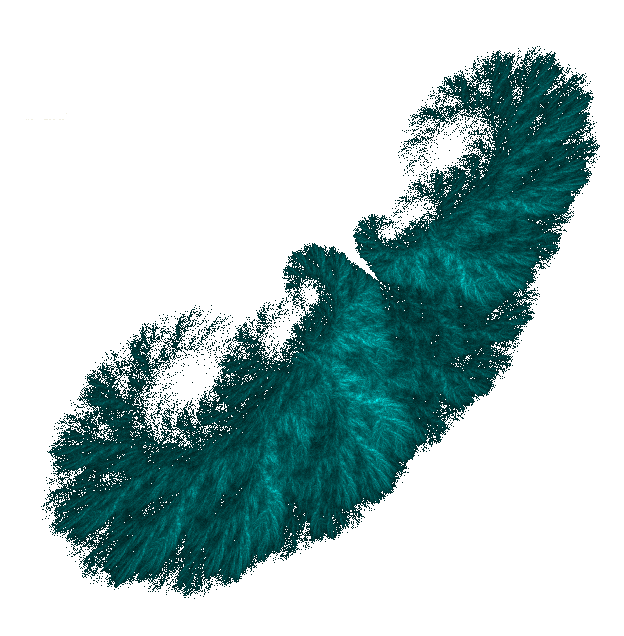
\includegraphics[width=\paperwidth,height=\paperheight,  keepaspectratio]{beamer1_biw.PNG}}
%
% \usebackgroundtemplate{\centering
%         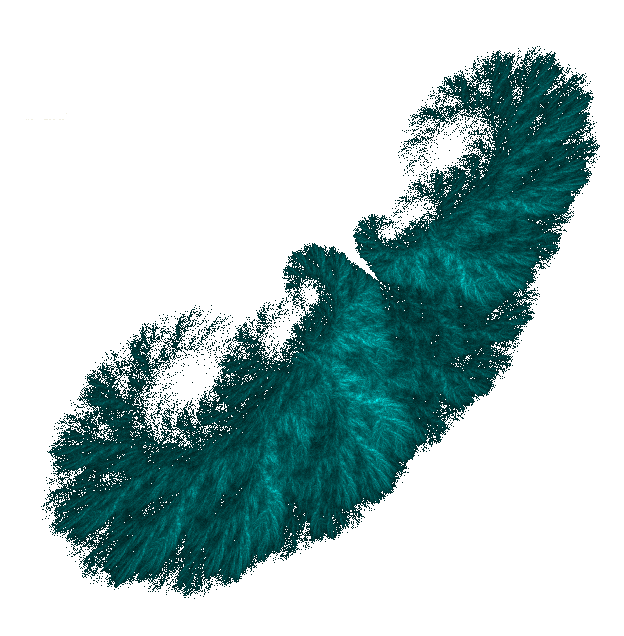
\includegraphics[height=7cm, keepaspectratio]{beamer1_biw.PNG}}

%\addtobeamertemplate{frame begin}{\pgfsetfillopacity{0.7}}{\pgfsetfillopacity{1}}
%\addtobeamertemplate{block begin}{\pgfsetfillopacity{0.7}}{\pgfsetfillopacity{1}}
% \title{Introduction to N-adic numbers}
% \subtitle{Practical Applications}
% \author{Denis Morozov}
% \institute{Samsung R\&D}
% \date{\today}

% %\setbeamercolor{color1}{fg = white}
% %\setbeamercolor{block title}{bg=red!30,fg=black}
% %\setbeamercolor{block body}{bg=red!30,fg=blue}

% \begin{document}

% \begin{frame}
% \titlepage
% \end{frame}

% \begin{frame}
% \begin{figure}[h]
% \center{\includegraphics[width=10em]{fomenko_solenoid.jpg}}
% \caption{A.Fomenko, 2-adic solenoid}
% \label{ris:image}
% \end{figure}
% %\centering \hspace{4em}\includegraphics[width=10em, keepaspectratio]{fomenko_solenoid.jpg}
% \end{frame}
% \begin{frame}
% \begin{block}{Introduction}

% \end{block}
% \end{frame}

% \end{document}
% $Header: /Users/joseph/Library/texmf/tex/latex/beamer/solutions/conference-talks/conference-ornate-20min.en.tex,v 90e850259b8b 2007/01/28 20:48:30 tantau $

\documentclass{beamer}

% This file is a solution template for:

% - Talk at a conference/colloquium.
% - Talk length is about 20min.
% - Style is ornate.



% Copyright 2004 by Till Tantau <tantau@users.sourceforge.net>.
%
% In principle, this file can be redistributed and/or modified under
% the terms of the GNU Public License, version 2.
%
% However, this file is supposed to be a template to be modified
% for your own needs. For this reason, if you use this file as a
% template and not specifically distribute it as part of a another
% package/program, I grant the extra permission to freely copy and
% modify this file as you see fit and even to delete this copyright
% notice. 


\mode<presentation>
{
  %\usetheme{CambridgeUS}
%\usetheme{Bergen}
%\usetheme{PaloAlto}
\usetheme{Warsaw}
  % or ...

  \setbeamercovered{transparent}
  % or whatever (possibly just delete it)
}


\usepackage[english]{babel}
% or whatever



\usepackage{times}
\usepackage[T1]{fontenc}
% Or whatever. Note that the encoding and the font should match. If T1
% does not look nice, try deleting the line with the fontenc.
%\usepackage{geometry} % to change the page dimensions
\usepackage{graphicx} % support the \includegraphics command and options
%\usepackage{pst-plot,pstricks-add}
%\usepackage[latin1]{inputenc}
\usepackage{tikz}

\usepackage{verbatim}
\usetikzlibrary{arrows,shapes}

% Курс нужен для более глубокого понимания работы процессора. Полученные знания могут быть использованы для оптимизации вычислительных алгоритмов.
% The course is necessary for a better understanding of the processor's work. The knowledge gained can be used to optimize the computational algorithms.
\title[Introduction to N-adic numbers] % (optional, use only with long paper titles)
{Introduction to N-adic numbers}

\subtitle
{Practical Applications}


\author[Denis Morozov, PhD \ Samsung R\&D] % (optional, use only with lots of authors)
{Denis~ Morozov, PhD  \\  \texttt{morozov.den@samsung.com}}
% - Give the names in the same order as the appear in the paper.
% - Use the \inst{?} command only if the authors have different
%   affiliation.
\institute[Samsung R\&D] % (optional, but mostly needed)
{
  \inst{1}%
  Samsung R\&D
  \and
  \inst{2}%
  Department of Computer Science, doctoral studies\\
  University of "Kiev-Mogyla Academy"}
%  \and
% \vspace{.5cm}
 % \inst{3}%
  % \texttt{ formulation of the problem}

  %  \texttt{Valentin Vovk},  \texttt{ Mobile Lab 2}}
% - Use the \inst command only if there are several affiliations.
% - Keep it simple, no one is interested in your street address.

\date[February, 2013] % (optional, should be abbreviation of conference name)
{Presentation , 2013}
% - Either use conference name or its abbreviation.
% - Not really informative to the audience, more for people (including
%   yourself) who are reading the slides online

\subject{N-adic numbers course}
% This is only inserted into the PDF information catalog. Can be left
% out. 

\AtBeginSubsection[]
{
  \begin{frame}<beamer>{Outline}
    \tableofcontents[currentsection,currentsubsection]
  \end{frame}
}


% If you wish to uncover everything in a step-wise fashion, uncomment
% the following command: 

%\beamerdefaultoverlayspecification{<+->}


\begin{document}


\begin{frame}
  \titlepage
\end{frame}

\begin{frame}
\begin{figure}[h]
\center{\includegraphics[width=11.5em]{fomenko_solenoid.jpg} }
\caption{A.Fomenko, 2-adic solenoid}
\label{ris:image}
\end{figure}
%\centering \hspace{4em}\includegraphics[width=10em, keepaspectratio]{fomenko_solenoid.jpg}
\end{frame}

\begin{frame}{Outline}
  \tableofcontents
  % You might wish to add the option [pausesections]
\end{frame}


% Structuring a talk is a difficult task and the following structure
% may not be suitable. Here are some rules that apply for this
% solution: 

% - Exactly two or three sections (other than the summary).
% - At *most* three subsections per section.
% - Talk about 30s to 2min per frame. So there should be between about
%   15 and 30 frames, all told.

% - A conference audience is likely to know very little of what you
%   are going to talk about. So *simplify*!
% - In a 20min talk, getting the main ideas across is hard
%   enough. Leave out details, even if it means being less precise than
%   you think necessary.
% - If you omit details that are vital to the proof/implementation,
%   just say so once. Everybody will be happy with that.

\section{Objective}

\subsection{Introduction}

\begin{frame}{Introduction}
N-adic analysis is key to understanding the logic of the processor.  
\pause

Not having deep understanding of the nature of the essences we work with, we have to strictly follow the rules that guarantee correct work results.
\pause

 However, the rules limit the range of solvable tasks, while violation of them may lead to an unpredictable result. Yet, such violation might be appropriate, given that we are fully aware of what we are doing.
\pause

Clear understanding of the nature of a processor's arithmetic is necessary for
building adequate computational models for problems encountered in the process of software development.
\end{frame}

%\end{block}

\subsection{Basic properties of ultrametrics}

\begin{frame}{Sufficiency}
  % - A title should summarize the slide in an understandable fashion
  %   for anyone how does not follow everything on the slide itself.
 Consideration for the following reasons ultrametrics (non-Archimedean metric spaces) is natural:
  \begin{itemize}
  \pause
  \item
in the context of a real analysis  the computer is a discrete system, but in terms of a 2-adic - continuous
     
  \pause
  \item
the modern computer is essentially an analog in terms of non Archimedean analysis
    
  \end{itemize}


\end{frame}

\begin{frame}{Quick calculations}
  % - A title should summarize the slide in an understandable fashion
  %   for anyone how does not follow everything on the slide itself.

 2-adic continuity of the processor's basic operations  allows the creation of models that use floating point numbers, but all calculations are made   in the set of integers.

 % \begin{itemize}
 % \pause
 %  \item

 % 32 bit integer algorithms have good specifications for optimizing on existing processors
 % \item
 % \pause
 % number-theoretical Fourier transform works well for convolutions with large kernels
 %  \end{itemize}

\end{frame}






\section{Description}

\subsection{Key components of the course}

\begin{frame}{Theory}
\pause
\begin{block}{Ultrametrics}
\pause
Basics of non Archimedean analysis. Ostrowski theorem.

\end{block}
\pause

\begin{block}{Izometries}
\pause
Izometrical polynomials of the ring $Z_2$. Inductive construction of isometries.
\end{block}
\pause
\begin{block}{Hensel's lemma}
\pause
Extend uniquely the root of polynomial in $\mathbb{Z}_p$ to of the root of a polynomial in $Z_p$.
\end{block}


\end{frame}



\begin{frame}{Practice}
\pause
\begin{block}{N-adic Arithmetics}
\pause
Basic of arithmetics of the ring $Z_2$ - addition, multiplication, division. 

\end{block}
\pause
\begin{block}{Presentation of real numbers in $Z_2$}
\pause
Rational numbers in $Z_2$. Some irrationals numbers in $Z_2$.
\end{block}
\pause
\begin{block}{Fast Calculations}
\pause
Using of 2-adic arithmetic for providing computational scheme close to the processor architecture.

\end{block}


\end{frame}
\subsection{Possible directions for further study}

\begin{frame}{Applications}

Using techniques discussed in the course is possible to build computational models that are close to the processor architecture.
\pause

 As a result, these models have good performance characteristics. Moreover we have no calculation errors that appear in the calculation with floating point.

\end{frame}



\begin{frame}{Links}

This course can be used as the basic for the course "Groups' automatous and the automorphisms' group of the regular
rooted tree "




\end{frame}

% \section*{Summary}

% \begin{frame}{Summary}

%   % Keep the summary *very short*.
%   \begin{itemize}
%   % \item
%   %   The \alert{first main message} of your talk in one or two lines.
%   \item
%     In this work implemented a two-dimensional integer convolution
% %\pause
%   \item
%     Possible sizes are - 2, 4, 8, 16, 32, 64, 128, 256, 512, 1024
%   \end{itemize}

%  \pause 
%   % The following outlook is optional.
%   \vskip0pt plus.5fill
%   \begin{itemize}
%   \item
%     Outlook
%     \begin{itemize}
%     \item
% Next task to investigate the possibility of constructing fast two-dimensional convolution for sizes that are not powers of two

%     \end{itemize}
%   \end{itemize}
% \end{frame}




% All of the following is optional and typically not needed. 
\appendix
\section<presentation>*{\appendixname}
\subsection<presentation>*{Bibliography}
\begin{frame}[allowframebreaks]
  \frametitle<presentation>{Bibliography}
    
  \begin{thebibliography}{3}
    
  \beamertemplatebookbibitems
  % Start with overview books.


  \bibitem{Govea1997}
    Fernando Q. Gouv\^ea 
    \newblock {\em P-Adic Numbers: An Introduction }.
    \newblock  Springer (1997)
 
    
 
  % Followed by interesting articles. Keep the list short. 

 \bibitem{  Koblitz1981}
 Nil  Koblitz
    \newblock {\em P-adic Numbers, p-adic Analysis, and Zeta-Functions }.
    \newblock  Mir (1981)
 
    
  \beamertemplatearticlebibitems
  % Followed by interesting articles. Keep the list short. 

  \bibitem{Morozov2011}
    Denis Morozov
    \newblock {\em  Differentiable finite-state izometries and izometric polynomials of the ring of
integer 2-adic numbers}.
    \newblock 8th Int.  Algebraic Conf.  in  Ukraine:  Abstr.
    \newblock Lugansk, July 2011

  \end{thebibliography}
\end{frame}
\end{document}



